\section{常规接触率和传播概率扩展}
\label{sec:sup:contact-scan}
\subsection{常规接触率的敏感性分析}
\label{sec:dom:c0}

固定西安传播参数 $\beta,\gamma,q_0$、$N_{\rm eff}=2\times10^4$、$\theta=0.002$（即 $\eta=40$）和绝对初值 $I_0=1.00659\times10^{-3}$，考察 $c_0$ 的影响。这里的 $c_0$ 是给定的常规接触水平，不作为额外控制量。

图~\ref{fig:c0-panel} 中，各控制轨迹的感染阈值相同。增大 $c_0$ 会使启动时间提前、最大隔离比例升高，与命题~\ref{prop:contact-effects} 一致。$c_0=3.43$ 时，$q_{\max}=0.383<\qinf=0.4119$，无内部拐点；$c_0=3.59$ 时，$q_{\max}=0.423$，内部拐点出现。存在拐点的各条轨迹均满足 $\qinf=0.4119$。


\begin{figure}[htbp]
\centering
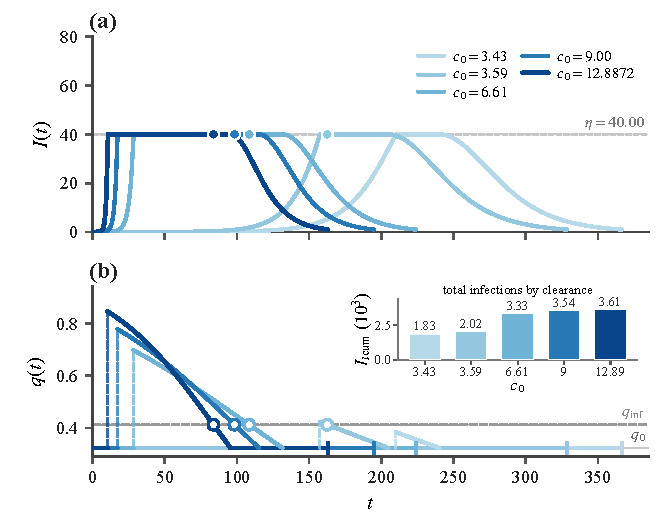
\includegraphics[width=112mm]{figures/layout_v5/c0_sensitivity_panel.pdf}
\caption{固定 $N_{\rm eff}=2\times10^4$、$\theta=0.002$，不同 $c_0$ 下的 (a) 感染人数和 (b) 隔离比例，横轴 $t$ 的单位为天。内嵌图为累计新增感染。$c_0=3.43$ 接近触发边界且无内部拐点；$c_0\approx6.61$ 对应控制时长的极大值，$c_0=12.8872$ 为基准接触率。存在内部拐点的曲线均满足 $\qinf=0.4119$。空心圆为隔离比例拐点，实心圆表示该时刻在感染曲线水平段上的位置，短竖线为清零时间。}
\label{fig:c0-panel}
\end{figure}


图~\ref{fig:c0-scan} 中，控制时长随 $c_0$ 先增加后减小，在 $c_0\approx6.61$ 时达到约 $103.2$ 天；成本和累计新增感染的极大值分别位于 $c_0\approx18.12$ 和 $13.88$，对应 $J\approx42.80$ 和 $\Itcum\approx3610$。三个极大值并不重合。

清零时间在所考察范围内随 $c_0$ 增大而减小，从 $c_0=3.43$ 时约 $367$ 天降至 $c_0=30$ 时约 $102$ 天。虽然控制时长在部分区间增加，但启动时间和退出后的下降时间缩短，使总时间减小。因此，控制时长不能单独决定清零时间。

图~\ref{fig:c0-phase} 给出 $(\theta,c_0)$ 平面上的触发边界、内部拐点边界和控制时长驻点曲线。三者分别对应控制是否启动、隔离比例是否存在内部拐点以及控制时长的变化方向。


\begin{figure}[htbp]
\centering
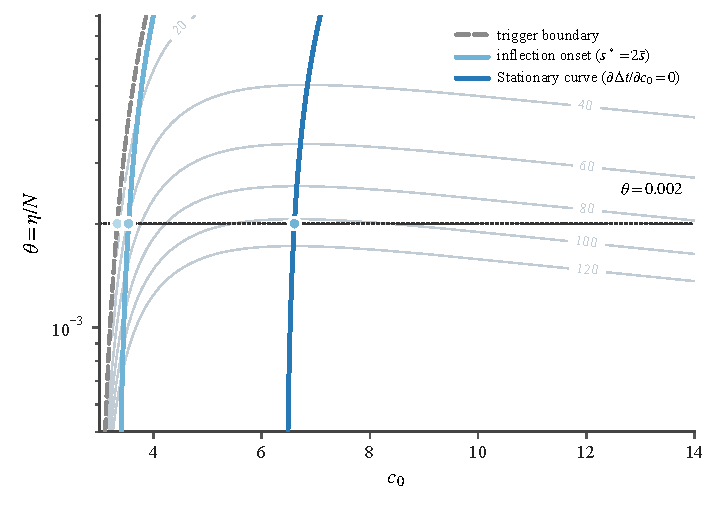
\includegraphics[width=120mm]{figures/layout_v5/c0_phase_stationary.pdf}
\caption{$(\theta,c_0)$ 平面上的触发边界、内部拐点边界 $s^*=2\bar s$ 和控制时长驻点曲线 $\partial\Delta t/\partial c_0=0$。灰色等值线表示控制时长，水平点线为 $\theta=0.002$。}
\label{fig:c0-phase}
\end{figure}


\subsection{常规接触率的敏感性分析}
\label{app:c0_scan}

固定 $N_{\rm eff}=2\times10^4$、$\theta=0.002$，图~\ref{fig:c0-scan} 给出各项指标随 $c_0$ 的变化。控制时长、成本与累计新增感染均存在数值极大值，其余时间指标在所考察范围内递减。

\begin{figure}[htbp]
    \centering
    \includegraphics[width=\textwidth]{c0_sensitivity_scan.pdf}
    \caption{固定 $N_{\rm eff}=2\times10^4$、$\theta=0.002$ 时各指标随 $c_0$ 的变化。(a)--(d) 依次为启动时间、控制时长、退出后的下降时间和清零时间；(e)--(h) 依次为最大隔离比例、拐点相对位置、成本和累计新增感染。竖线标示触发边界 $3.334$、拐点边界 $3.543$ 和时长极大值位置 $6.607$。}
    \label{fig:c0-scan}
\end{figure}


\subsection{接触率与传播概率对拐点存在性的影响}
\label{app:c0_beta}

固定 $\theta=0.002$、$q_0=0.3230$ 及绝对初值，图~\ref{fig:c0-beta-existence} 给出 $(c_0,\beta)$ 平面上满足 $s_c<2\bar s<s^*$ 的参数范围。西安参数 $(12.8872,0.1498)$ 位于内部拐点存在区域内。

\begin{figure}[htbp]
    \centering
    \includegraphics[width=0.7\textwidth]{c0_beta_existence.pdf}
    \caption{固定 $\theta=0.002$、$q_0=0.3230$ 时，$(c_0,\beta)$ 平面上的内部拐点存在范围。边界为 $2\bar s=s^*$ 和 $\beta_{\max}=0.2614$，标记点为西安参数 $(12.8872,0.1498)$。}
    \label{fig:c0-beta-existence}
\end{figure}

\FloatBarrier

% 参考文献


\FloatBarrier

